\documentclass[10pt,a4paper, titlepage]{article}
\usepackage[spanish]{babel}
\usepackage[utf8]{inputenc}
\usepackage{amsmath}
\usepackage{amsfonts}
\usepackage{amssymb}
\usepackage{eurosym}

\usepackage{hyperref}
\hypersetup{
    colorlinks=true,
    linkcolor=black,
    filecolor=black,
    urlcolor=cyan,
}

\urlstyle{same}


\usepackage{graphicx}
\usepackage{caption}
\usepackage{subcaption}

\usepackage[margin=0.9in]{geometry}
\usepackage[stable]{footmisc}

\spanishdecimal{.}

\title{\textbf{Resumen sobre Información\\de Empresa Telefónica}}
\author{Carlos Solsona Álvarez\\Cesar Torres Martinez\\Javier García Seller\\Oskar Denis Siodmok\\Steven Adrados Khunliang}

\begin{document}
\maketitle
\pagebreak
\section{Introducción}
Se quiere realizar un estudio de los datos de una empresa telefónica para el cual se ha proporcionado una hoja de datos con una muestra de 188 clientes.
En concreto, con los siguientes tipos de datos: género, permanencia, coste mensual, coste acumulado, servicio telefónico y servicio de internet.

\section{Análisis de la permanencia y edad de los clientes}
Realizado un análisis de la permanencia (en meses) de los clientes, se observa que la empresa presenta pérdidas abruptas de clientes a partir de los 10 meses, aun así esta pérdida no supone ni un cuarto de los clientes totales (figura \ref{fig:per-freq-pie}) ya que la mayoría permanece con la compañía. Tras este umbral los clientes se mantienen constantes con el paso del tiempo con una mayor estabilidad entre los 40 y 70 meses (figura \ref{fig:per-freq-hist}). Respecto a la edad de los clientes, existe una gran dispersión aunque la gran mayoría se agrupa entre los 35 y 65 años (figura \ref{fig:age-box}).
\begin{figure}[!htb]
\minipage{0.32\textwidth}
  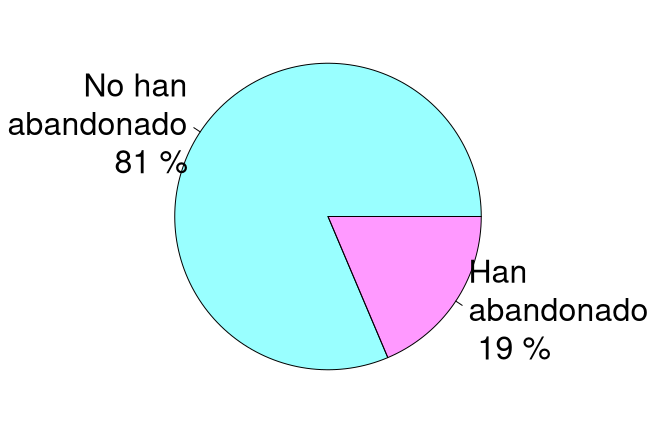
\includegraphics[width=\linewidth]{per-freq-pie}
  \caption{Proporción de clientes que han abandonado.}\label{fig:per-freq-pie}
\endminipage\hfill
\minipage{0.32\textwidth}
  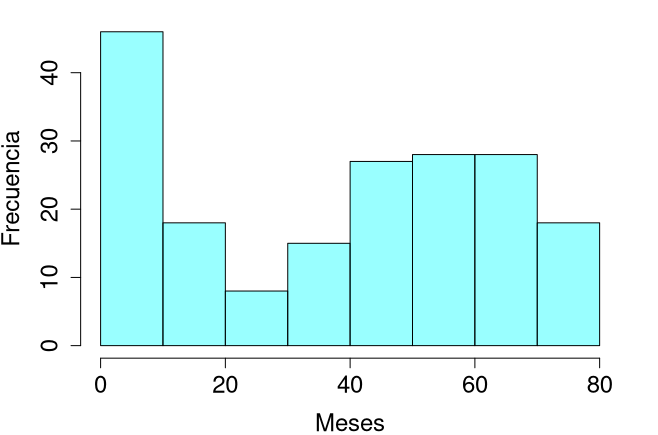
\includegraphics[width=\linewidth]{per-freq-hist}
  \caption{Histograma de la pertenencia según los meses.}\label{fig:per-freq-hist}
\endminipage\hfill
\minipage{0.32\textwidth}
  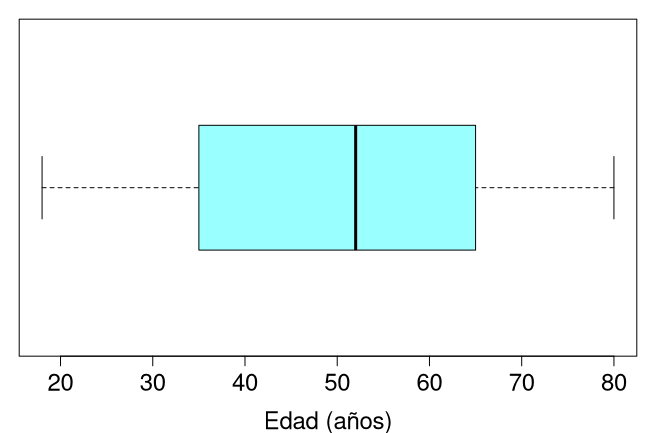
\includegraphics[width=\linewidth]{age-box}
  \caption{Diagrama de cajas de la edad de los clientes.}\label{fig:age-box}
\endminipage\hfill
\end{figure}

No sería prudente justificar los abandonos con los precios ya que estos se mantienen cerca de la media (como se observa en la figuras \ref{fig:month-churn-box} y \ref{fig:total-churn-box}). Esto sugiere que los abandonos son causados por otros factores.
\begin{figure}[!htb]
     \centering
     \begin{subfigure}[b]{0.4\textwidth}
         \centering
         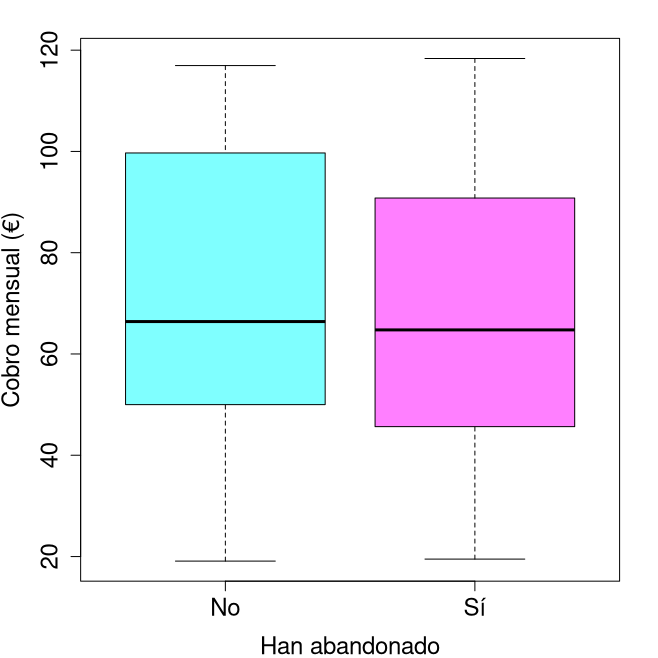
\includegraphics[width=\textwidth]{month-churn-box}
         \caption{Cobros mensuales.}
		 \label{fig:month-churn-box}
	 \end{subfigure}\hspace{1cm}
     \begin{subfigure}[b]{0.4\textwidth}
         \centering
         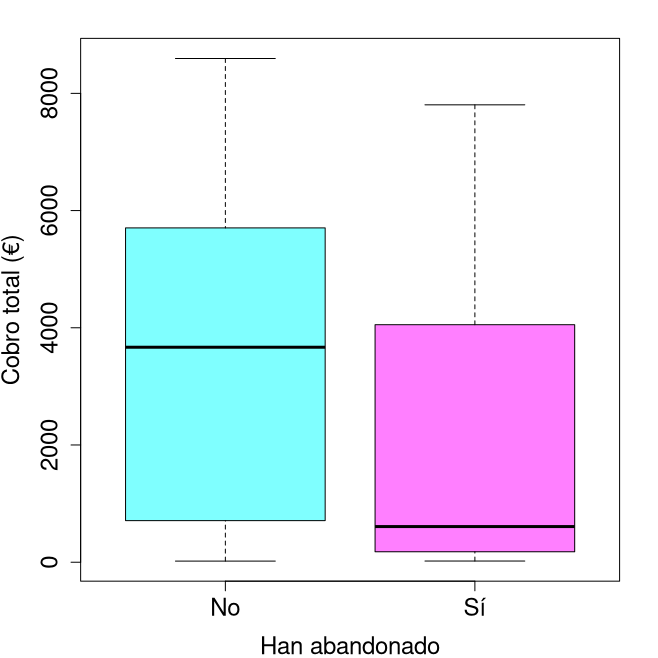
\includegraphics[width=\textwidth]{total-churn-box}
         \caption{Cobros acumulados.}
		 \label{fig:total-churn-box}
     \end{subfigure}
        \caption{Diagramas de cajas de los cobros de los clientes según si han abandonado o no.}
		\label{fig:churns-box}
\end{figure}
\section{Análisis de servicios contratados}
Como se observa en la figura \ref{fig: phone-pie}, la mayoría de clientes tienen un móvil contratado. Lo mismo pasa con el internet. Aun así, entre ADSL y Fibra óptica hay una diferencia mínima de clientes (figura \ref{fig: net-pie}). 
\begin{figure}[!htb]
	\centering
   \begin{minipage}{0.41\textwidth}
     \centering
     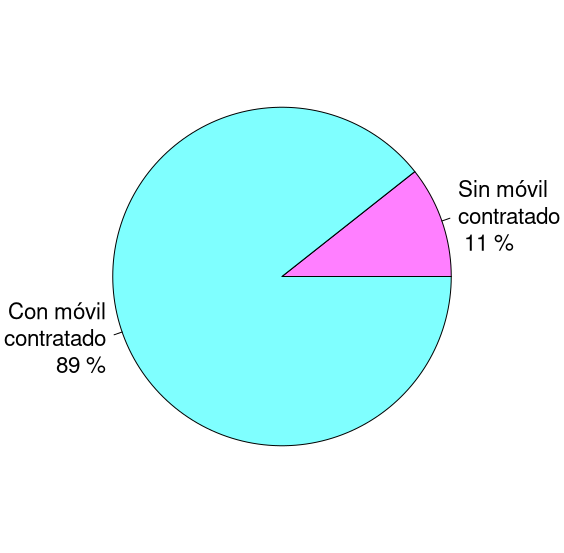
\includegraphics[width=\linewidth]{phone-pie}
     \caption{Proporicón de clientes del servicio móvil}\label{fig: phone-pie}
 \end{minipage}\hspace{1cm}
   \begin{minipage}{0.41\textwidth}
     \centering
     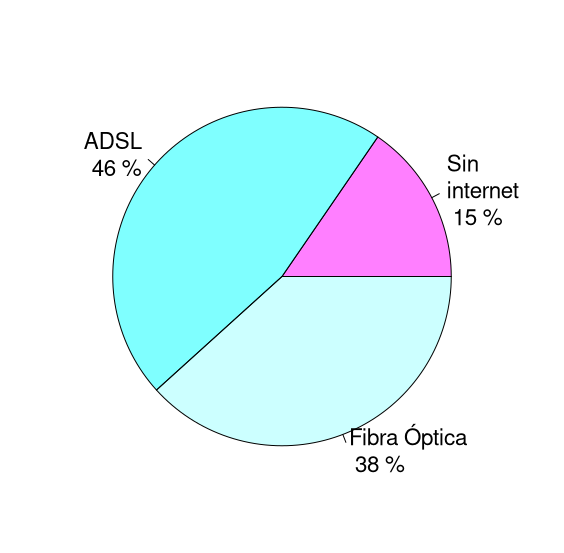
\includegraphics[width=\linewidth]{net-pie}
     \caption{Proporicón de tipos de red contratados.}\label{fig: net-pie}
   \end{minipage}
\end{figure}
\begin{figure}[!htb]
	\centering
   \begin{minipage}{0.41\textwidth}
     \centering
     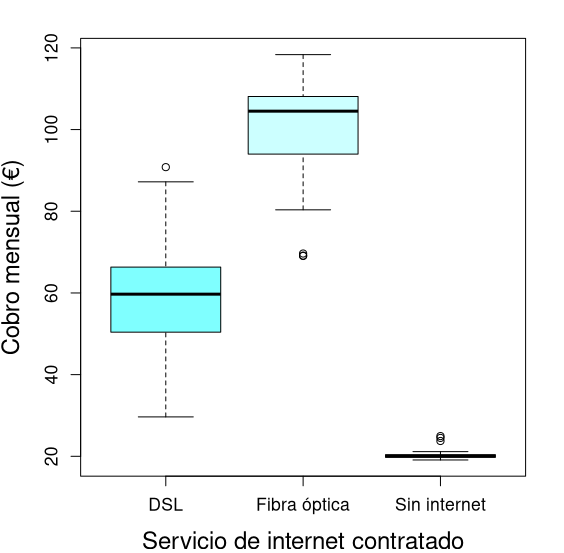
\includegraphics[width=\linewidth]{net-box}
     \caption{Proporicón de clientes del servicio móvil}\label{fig: net-box}
 \end{minipage}\hspace{1cm}
   \begin{minipage}{0.41\textwidth}
     \centering
     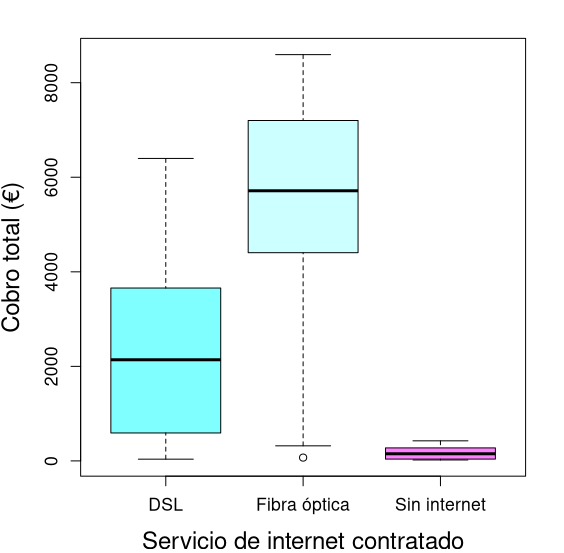
\includegraphics[width=\linewidth]{net-total-box}
     \caption{Proporicón de tipos de red contratados.}\label{fig: net-total-box}
   \end{minipage}
\end{figure}
Entre las posibles causas de este hecho, especulamos que podría deberse a la baja disponibilidad de la fibra o debido al precio más competitivo del ADSL, como se observa en las figuras \ref{fig: net-box} y \ref{fig: net-total-box}.

\section{Análisis de cobros} 
Con respecto a los pagos, mensualmente hay una notable dispersión de las cantidades pagadas por los clientes destacando que una gran mayoría de estos se encuentran en el rango de  50 y 100 \euro{} (figura \ref{fig: month-box}). De forma acumulada los pagos más comunes llegan a 1000 \euro{} posteriormente estabilizandose en el rango de 1000 y 8000 \euro{} llegando a un máximo en 4500 \euro{} (figura \ref{fig: total-hist}). 

Respecto al cobro según el género se observa que por lo general las mujeres pagan una cantidad ligeramente mayor que los hombres tanto de manera mensual como acumulada (figura \ref{fig:gen-box}).
\begin{figure}[!htb]
   \begin{minipage}{0.48\textwidth}
     \centering
     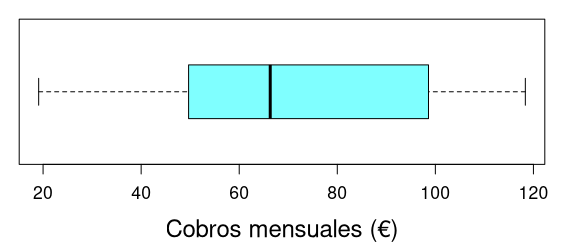
\includegraphics[width=\linewidth]{month-box}
     \caption{Diagrama de cajas de los cobros.}\label{fig: month-box}
   \end{minipage}\hfill
   \begin{minipage}{0.48\textwidth}
     \centering
     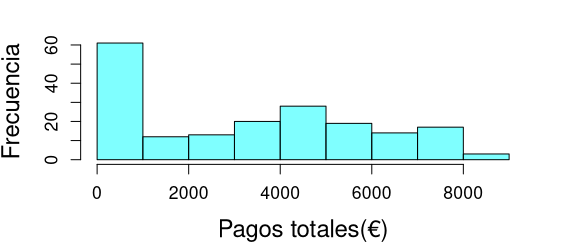
\includegraphics[width=\linewidth]{total-hist}
     \caption{Histograma del cobro acumulado.}\label{fig: total-hist}
   \end{minipage}
\end{figure}

\begin{figure}[!htb]
     \centering
     \begin{subfigure}[b]{0.4\textwidth}
         \centering
         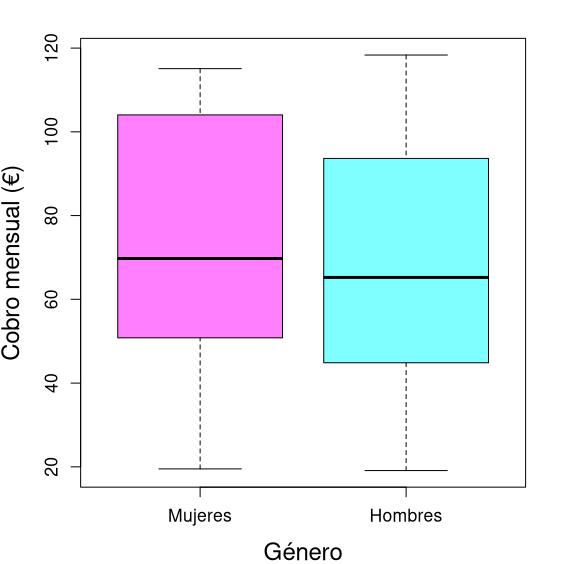
\includegraphics[width=\textwidth]{month-gen-box}
         \caption{Cobros mensuales.}
		 \label{fig:month-gen-box}
	 \end{subfigure}\hspace{1cm}
     \begin{subfigure}[b]{0.4\textwidth}
         \centering
         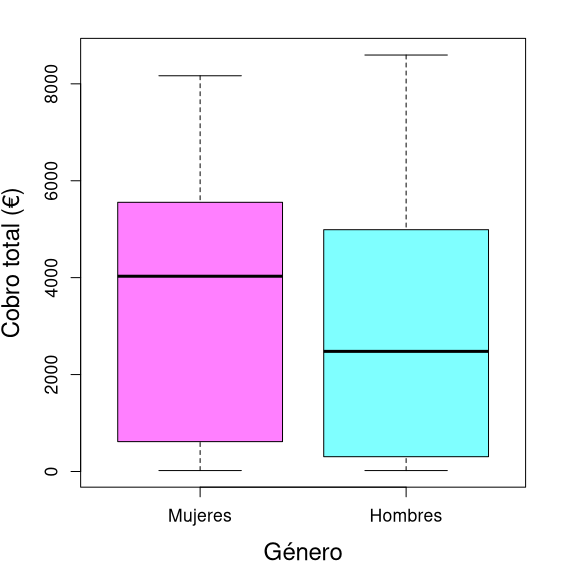
\includegraphics[width=\textwidth]{total-gen-box}
         \caption{Cobros acumulados.}
		 \label{fig:total-gen-box}
     \end{subfigure}
        \caption{Diagramas de cajas de los cobros de los clientes según su género.}
		\label{fig:gen-box}
\end{figure}
Con el análisis de la permanencia en meses de los clientes junto a sus cobros (figura \ref{fig: month-churn}) distinguimos dos principales tipos de clientes, un primer grupo que tiende una permanencia más bien corta con pagos entre bajos y moderados y un segundo grupo con altos pagos y larga permanencia. Distinguiendo el género (figura \ref{fig: month-churn-gen}) se llega a la conclusión que las mujeres generalmente pagan más que los hombres con una diferencia de un pequeño umbral. Bajo el mismo razonamiento, por lo general, las mujeres son más propensas a abandonar la compañía ante un mismo cobro mensual, otra vez con una diferencia casi mínima.
\begin{figure}[!htb]
   \begin{minipage}{0.48\textwidth}
     \centering
     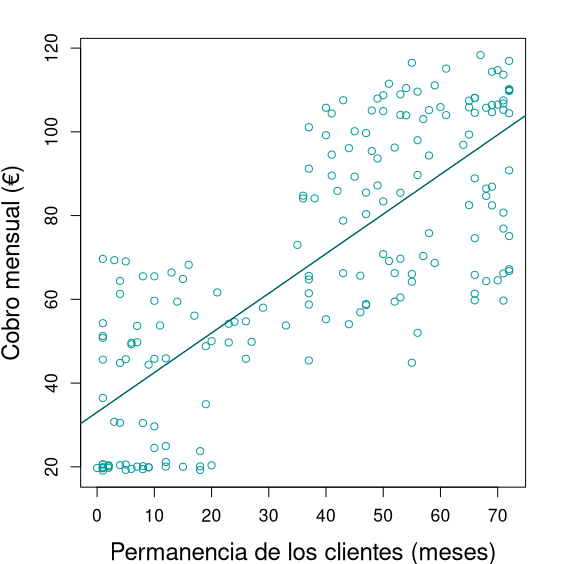
\includegraphics[width=\linewidth]{month-churn}
	 \caption{Relación entre los abandonos de los clientes respecto a sus cobros mensuales.}\label{fig: month-churn}
   \end{minipage}\hfill
   \begin{minipage}{0.48\textwidth}
     \centering
     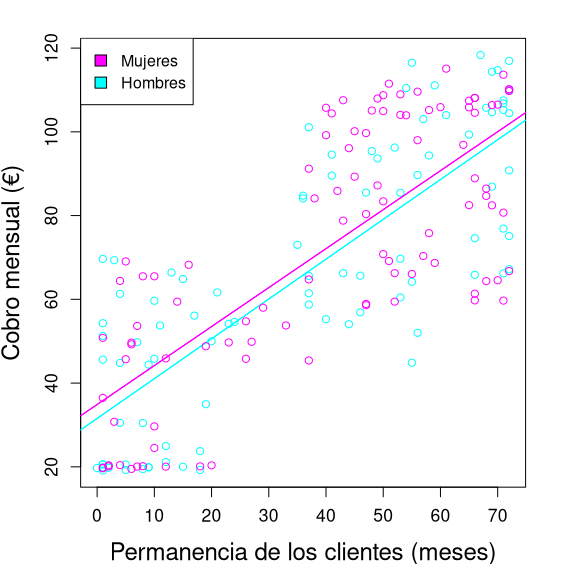
\includegraphics[width=\linewidth]{month-churn-gen}
     \caption{Relación entre cobros mensuales y permanencia pero distinguiendo el género.}\label{fig: month-churn-gen}
   \end{minipage}
\end{figure}
\section{Anexo}
Código fuente: \url{https://github.com/Denis-urjc/estadistica-practica1-codigo-fuente}
\end{document}
